\documentclass{sigchi}

% Use this command to override the default ACM copyright statement
% (e.g. for preprints).  Consult the conference website for the
% camera-ready copyright statement.

%% EXAMPLE BEGIN -- HOW TO OVERRIDE THE DEFAULT COPYRIGHT STRIP -- (July 22, 2013 - Paul Baumann)
% \toappear{Permission to make digital or hard copies of all or part of this work for personal or classroom use is      granted without fee provided that copies are not made or distributed for profit or commercial advantage and that copies bear this notice and the full citation on the first page. Copyrights for components of this work owned by others than ACM must be honored. Abstracting with credit is permitted. To copy otherwise, or republish, to post on servers or to redistribute to lists, requires prior specific permission and/or a fee. Request permissions from permissions@acm.org. \\
% {\emph{CHI'14}}, April 26--May 1, 2014, Toronto, Canada. \\
% Copyright \copyright~2014 ACM ISBN/14/04...\$15.00. \\
% DOI string from ACM form confirmation}
%% EXAMPLE END -- HOW TO OVERRIDE THE DEFAULT COPYRIGHT STRIP -- (July 22, 2013 - Paul Baumann)

% Arabic page numbers for submission.  Remove this line to eliminate
% page numbers for the camera ready copy
% \pagenumbering{arabic}

% Load basic packages
\usepackage{balance}  % to better equalize the last page
\usepackage{graphics} % for EPS, load graphicx instead 
\usepackage[T1]{fontenc}
\usepackage{txfonts}
\usepackage{mathptmx}
\usepackage[pdftex]{hyperref}
\usepackage{color}
\usepackage{booktabs}
\usepackage{textcomp}
\usepackage{multicol}
% Some optional stuff you might like/need.
\usepackage{microtype} % Improved Tracking and Kerning
% \usepackage[all]{hypcap}  % Fixes bug in hyperref caption linking
\usepackage{ccicons}  % Cite your images correctly!
% \usepackage[utf8]{inputenc} % for a UTF8 editor only

% If you want to use todo notes, marginpars etc. during creation of your draft document, you
% have to enable the "chi_draft" option for the document class. To do this, change the very first
% line to: "\documentclass[chi_draft]{sigchi}". You can then place todo notes by using the "\todo{...}"
% command. Make sure to disable the draft option again before submitting your final document.
\usepackage{todonotes}

% Paper metadata (use plain text, for PDF inclusion and later
% re-using, if desired).  Use \emtpyauthor when submitting for review
% so you remain anonymous.
\def\plaintitle{Synthetic Interviewing with Semantic Search}
\def\plainauthor{First Author, Second Author, Third Author,
  Fourth Author, Fifth Author, Sixth Author}
\def\emptyauthor{}
\def\plainkeywords{Authors' choice; of terms; separated; by
  semicolons; include commas, within terms only; required.}
\def\plaingeneralterms{Documentation, Standardization}

% llt: Define a global style for URLs, rather that the default one
\makeatletter
\def\url@leostyle{%
  \@ifundefined{selectfont}{
    \def\UrlFont{\sf}
  }{
    \def\UrlFont{\small\bf\ttfamily}
  }}
\makeatother
\urlstyle{leo}

% To make various LaTeX processors do the right thing with page size.
\def\pprw{8.5in}
\def\pprh{11in}
\special{papersize=\pprw,\pprh}
\setlength{\paperwidth}{\pprw}
\setlength{\paperheight}{\pprh}
\setlength{\pdfpagewidth}{\pprw}
\setlength{\pdfpageheight}{\pprh}

% Make sure hyperref comes last of your loaded packages, to give it a
% fighting chance of not being over-written, since its job is to
% redefine many LaTeX commands.
\definecolor{linkColor}{RGB}{6,125,233}
\hypersetup{%
  pdftitle={\plaintitle},
% Use \plainauthor for final version.
%  pdfauthor={\plainauthor},
  pdfauthor={\emptyauthor},
  pdfkeywords={\plainkeywords},
  bookmarksnumbered,
  pdfstartview={FitH},
  colorlinks,
  citecolor=black,
  filecolor=black,
  linkcolor=black,
  urlcolor=linkColor,
  breaklinks=true,
}

% create a shortcut to typeset table andings
% \newcommand\tabhead[1]{\small\textbf{#1}}

% End of preamble. Here it comes the document.
\begin{document}

\title{\plaintitle}

\numberofauthors{3}
\author{%
  \alignauthor{Leave Authors Anonymous\\
    \affaddr{for Submission}\\
    \affaddr{City, Country}\\
    \email{e-mail address}}\\
  \alignauthor{Leave Authors Anonymous\\
    \affaddr{for Submission}\\
    \affaddr{City, Country}\\
    \email{e-mail address}}\\
  \alignauthor{Leave Authors Anonymous\\
    \affaddr{for Submission}\\
    \affaddr{City, Country}\\
    \email{e-mail address}}\\
}

\maketitle

\begin{abstract}
  In this paper we describe a novel tool to open up new windows of exploration for qualitative researchers. Through the use of semantic search algorithms applied to a large corpus of data, obtained from LiveJournal.com, we are able to extract valuable information that qualitative researchers can use in their methodology. We describe the design processes that lead us to the development of this tool. We analyze the results of an open user study with qualitative researchers, which helped us confirm the value of the tool and lead to the development of additional features. Finally we present comparisons between results obtained by modifying certain input parameters such as: percentage of data used, number of results returned, filtering, and word weighting.
\end{abstract}

\category{H.3.3}{Information Search and Retrieval}{}
\category{J.4}{Social and Behavioral Sciences}{}
\category{H.5.m.}{Information Interfaces and Presentation  (e.g. HCI)}{Miscellaneous} 

\keywords{semantic search; big data; qualitative; ethnography; synthetic; methods}

\section{Introduction}

Semi-structured interviews are a central tool in user research and the social sciences more generally.
They allow for rich and open-ended exploration of user attitudes, preferences, desires, fears and values. 
While they are of tremendous value, they also have difficulties:

\begin{itemize}
\item They are expensive in time and resources. They often involve travel by one or both parties,
  recording and transcription of content, subject reimbursement, and later effort by the interviewer
  to form a synthesis from individual interviews.
\item They are real-time which affords continuity in the thoughts of the interviewee, but also challenges
  the interviewer to decide instantly what topics to pursue.
\item They typically involve a relatively small sample of subjects. While one obtains a breadth of
  responses it is difficult to know how widely-shared these are.
\item They are normally time-bounded. Parties make a prior commitment to the duration of the interview,
  which cannot be adjusted to follow promising threads that emerge late in the interview.
\end{itemize}

In this paper, we explore the use of Big Data technologies to provide an alternative to
semi-structured interviews that serves some of the same goals. Specifically we explore recently
developed deep semantic embedding techniques to discover relevant posts from a large corpus of
user-generated content. We use a corpus of public posts from the LiveJournal site.  LiveJournal is a
social media site where users maintain a personal online journal or diary. LiveJournal posts tend to
be longer than other sites, and the journal format encourages externalization of user attitudes and
values. Explicit sentiment is attached to some posts via an emoticon system. The site contains many
themed areas around topics such as health and lifestyle.  Even among the public posts there are many
where users discuss significantly life challenges and seek and provide support for others. The
content does not cover every possible topic, but the corpus is quite large and rich and coverage of
rarer topics grows as the corpus grows.  We describe a tool which allows an ``interviewer'' to
explore this corpus via a series of ``questions'' similar to a semi-structured interview. Each
question retrieves a set of relevant sentences from various parts of the corpus, and the containing
posts can be retrieved to provide context around them.

Within the LiveJournal corpus are significant tracts of text where users discuss attitudes, values
and personal experiences around various topics. We argue that these tracts are similar to the
responses users might give in a semi-structured interview. They even occur in the context of that
user's history of posts, which can be explored to better understand their background. The challenge
then is to separate the relevant tracts from other parts of the corpus. This is where deep semantic
technologies come in. Word2vec is a neural semantic embedding method that has been shown to perform
well at a variety of semantic tasks. ``Semantics'' here includes not just propositional content,
but sentiment and even style. We argue that use of these technologies provides a much richer form
of matching than traditional keyword-based search and even first-generation semantic search
techniques such as Latent Semantic Indexing (LSI). We bolster this argument with our experiments
which showed that perceived quality of the retrieved results was improved by {\em filtering out}
surface-matching (i.e. keyword-matching) posts from semantically-matching posts.

While this approach is not a replacement for semi-structured interviews, it can serve some of the
same goals. This is especially true for topics that are more general and therefore well-covered in
the corpus. For these topics, there are potential advantages of this approach over classical
interviews, which include:

\begin{description}
\item[Economy] Our approach is very economical compared to live interviews. No travel is involved,
  no transcription, no subject payments.
\item[Interviewer Reflection] Interviewers can take as much time as needed to compose questions.
  There is no cost to pursuing side themes, or with ``dead-end'' themes. Interviews can last as long
  as desired, be paused/restarted etc. 
\item[Representativeness/Diversity] The number of users who will post about a popular topic (e.g. health,
  transportation) is large compared to the number of users who would be involved in face-to-face
  interviews. By exploring up and down the set of relevant sentences, the interviewer gains a
  sense of typical attitudes.
\item[Interviewer Control] Our system provides a variety of controls and filters over the retrieved
  results. With practice, this allows the interviewer to more quickly get the kinds of responses
  they are looking for, compared to reformulating questions in a live interview. 
\end{description}

We present evidence that the value of this approach improves with the size of the corpus and the
effectiveness of the semantic embedding method. With the recent rapid progress in scalability and
accuracy of semantic embedding methods, this means that our approach will improve in usefulness
with these developments. 

\section{related work}

Keyword searches were the first approach to mining a large corpus of data for relevant information. Exploration techniques using single-word queries date back to keyword-in-context indexing (KWIC) \cite{luhn60, fischer66} which provides snippets of text surrounding the search query and a key for reading the text in its original context. This model is still relevant, but the results are difficult to parse and recent work has focused on visualization methods such as Word Tree \cite{wattenberg08} which aggregates results with identical word sequences and displays them in a tree-like structure. Later visual text exploration tools based on the Word Tree visualization paradigm include WordSeer \cite{muralidharan13}  which makes it easier to navigate a corpus by facilitating switching between different views, adding summary statistics and applying filters (such as date ranges or other metadata). Other refinements included imposing specific grammatical requirements on the results \cite{muralidharan13b}.\\

A standard goal of semi-structured interviews is to obtain non-obvious insights, responses pertinent to the original topic but not expected by the interviewer. Most such interview responses are not expected to explicitly contain words from the interviewer's questions. For this purpose, keyword search techniques can be too restrictive. Some efforts have been made to search a corpus directly by document level themes. One such example provides a flexible visualization and exploration tool \cite{eisenstein12} based on topic modeling, a technique to identify latent themes across a collection of documents~\cite{blei12}. As an alternative to the latent concept approach, the relatedness of texts has also been computed using explicit semantic analysis on natural concepts as defined by humans via Wikipedia~\cite{gabrilovich07}. Another attempt to leverage the Wikipedia corpus for semantic annotation of content is described in~\cite{mihalcea07}.

Researchers have also made efforts to developing a semantic similarity metric applicable at the word or sentence level. Schemes for measuring similarity at the word level include LSI and Pointwise Mutual Information and Information Retrieval (PMI-IR)~\cite{turney2001}, both of which learn semantic relationships based on co-occurrence of words in a training corpus. More recently, distributed word embeddings learned with recurrent neural networks have become state of the art through algorithms like word2vec, which we use here and describe in the Methodology section. Building on these efforts, various models to compute short text similarity  based on  word-level semantic similarity were also developed~\cite{mihalcea2006,kenter15short}. A recent paper also attempts to develop direct embeddings at the sentence level using long short term memory (LSTM) neural networks, called skip-thought vectors~\cite{kiros2015skip}. 

\section{Methodology}

\subsection{LiveJournal Corpus}
For this study, we obtained a data set consisting of all LiveJournal posts as of November 2012 in raw XML format. As previously mentioned, LiveJournal is a social networking service where users can keep a blog, journal, or diary. Users have their own journal pages, which show all of their most recent journal entries. Each journal entry can also be viewed on its own web page which includes comments left by other users. 

As of 2012, LiveJournal in the United States received about 170 million page views each month from 10 million unique visitors. Our data contains about one million users with a total of 64,326,865 text posts. Of the users that provided their date of birth, the majority were in the 17-25 age group. Additionally, users were able to indicate their binary gender; of those who did so 45\% identified as male and 55\% as female. 

The median sentence length is 10 and, as expected, the distribution of sentence lengths follows a power law.

\begin{figure}[tb]
\centering 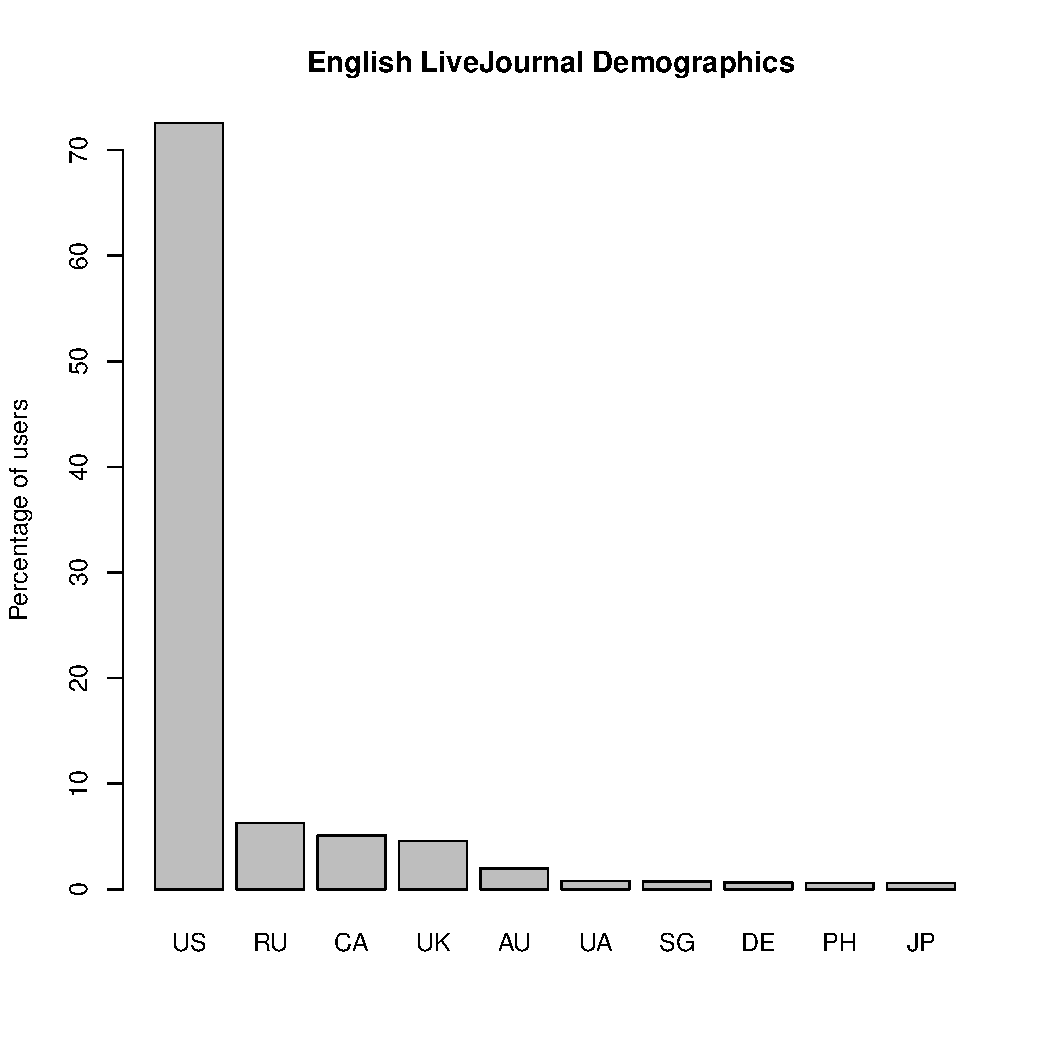
\includegraphics[width=0.3\textwidth]{figures/demographics} 
\caption{The representation of the top 10 countries in our data set.  \label{fig:demographics}}
\end{figure}


\subsection{Data preprocessing}

We started with a raw XML dataset which consists of more than 9 billion words in over 500 million sentences. In order to extract semantic meaning and run synthetic interviews through the use of natural language processing (NLP) algorithms, we implemented a data pipeline that allows us to extract and clean the post text in a computationally efficient form. 

The first step is to tokenize the corpus using FLEX (Fast Lexical Analyzer), a scanner which maps each word in the corpus to a unique number and saves the mapping in a dictionary. For efficiency, we keep only the 994,949 most common words and discard the rest (all of which occur fewer than 41 times in the entire dataset). Care is taken to properly tokenize numbers and emoticons such as ``:-)'', ``=<'' or ``>:P''.

After removing non-textual content such as images, hyperlinks, and XML formatting data, a bag-of-words (BOW) representation is saved for each sentence from the posts as a column in a sparse feature matrix. The rows of this matrix correspond to the entries in the dictionary above, and the values in the matrix are the counts of each entry for each sentence. For each sentence, we also store the ID of the post it belongs to and the user who wrote it so that the original post can be found online. Finally, we keep the tokenized sentence data in order to display results when performing the query.

%The first thing we implemented was Lucene search into our dataset. This allowed us to first actually see what users were writing and with what moods. UCSF School of Nursing has a life events questionnaire detailing < http://nursing.ucsf.edu/sites/nursing.ucsf.edu/files/LifeEventsQues.pdf> ten categories of life events that may bring about changes in the lives of those who experience them. Some major categories are health, work, love and marriage, family and close friends, personal and social. We wanted to search through the data and see the posts relating to major life events such as disease, cancer, and others. 

\subsection{word2vec}
We explore synthetic interviewing by employing word2vec \cite{Mikolov2013,MikolovSCCD13}, a popular word embedding model which has been successful in a variety of NLP applications, including analogy tasks, sentence completion, machine translation \cite{W15-4908}, and topic modeling \cite{djuric2015hierarchical}. Word embedding models map each dictionary word into a lower dimensional continuous vector representation. With word2vec, this embedding is learned automatically from a sample corpus using a recurrent neural network. 

The true power of the technique is that the resulting feature space demonstrates semantic structure, e.g. $\text{vec(``king'')}\,{-}\, \text{vec(``man'')}\,{+}\,\text{vec(``woman'')}$ has a greater cosine similarity to vec(``queen'') than to the vector of any other word in the dictionary. We can also generalize this comparison technique beyond the scope of single-words. By performing vector addition on the word vector embeddings of corresponding words and normalizing the resulting sum, we can compare the semantic proximity of complete sentences. This procedure is described in detail below.

We use two embedding models trained on two different corpus. First, we train our own embedding model on the corpus of LiveJournal posts using the Skip-gram with negative sampling (SGNS) implementation of word2vec as recommended in \cite{MikolovSCCD13}. This model gives 300-dimensional embeddings for the 994,949 words in our dictionary. Conveniently, Mikolov et.~al published a pre-trained SGNS word2vec model for open source access \cite{word2vecWEB}. This model was trained on a 100 billion-word Google News corpus, and gives 300-dimensional embeddings for 3 million unique words. All of the words from our LiveJournal dictionary that are not included in this model are mapped to zero vectors. Common stop words (i.e. ``the'', ``an'', ``who'') provide little semantic information and are also mapped to zero vectors.

%\begin{figure}[tb]
%\centering 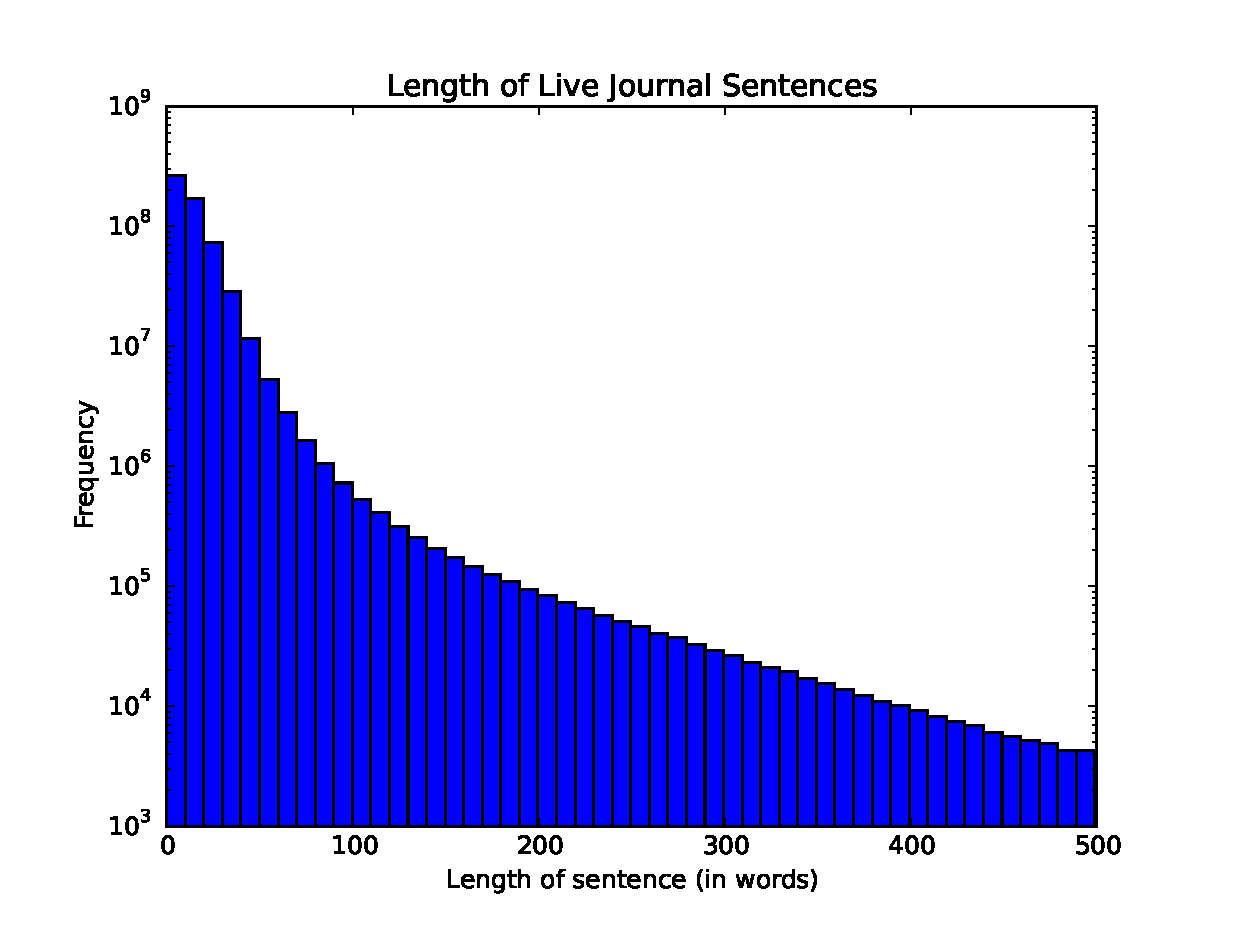
\includegraphics[width=0.5\textwidth]{figures/LJCounts} 
%\caption{Histogram of the distribution of sentence lengths in the LiveJournal dataset. \label{fig:wordCounts}}
%\end{figure}

%\begin{figure}[tb]
%\centering 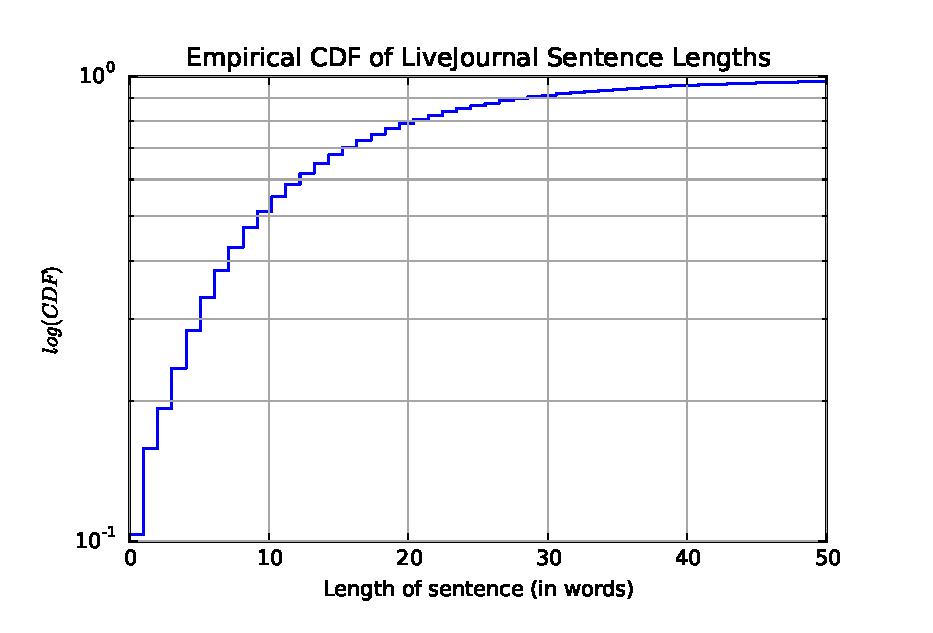
\includegraphics[width=0.4\textwidth]{figures/wordCDF} 
%\caption{Cumulative distribution function (CDF) for the distribution of sentence lengths in the LiveJournal dataset which represents the percentage of sentences containing less than a given number of words. Note that the $y$-axis is logarithmic and the median sentence length is 10 words. \label{fig:wordCDF}}
%\end{figure}

\subsection{Querying}

The goal is to perform semantic searches on the dataset from queries which can range from individual words to full sentences. To do this, we find the similarity of sentences based on the embeddings of their individual words. Specifically, we define a sentence embedding to be the mean of its constituent word vector embeddings. The interviewer's question is also converted to a sentence embedding and tested on the data set using cosine similarity. Note that multi-sentence queries are also possible by treating the entire query in the same way. Word embeddings have been employed in more recent and sophisticated approaches, which outperform our similarity method when used in short text strings \cite{kenter15short}. However, our approach has sufficient power for our goal while favoring rapid retrieval of the best matches from a large corpus. 
%The goal is to perform semantic searches on the dataset from queries which can range from individual words to full sen- tences. To do this, we require a procedure for finding the similarity of sentences based on the embeddings of the individ- ual words. A simple choice is to embedded as the mean of the constituent word vector embeddings. The question is posed to the data set using the cosine similarity in this embedding.

In order to query the data, we multiply the word2vec embedding matrix and the sparse bag of words matrix described above to get a semantic matrix. Each column of this matrix is the word2vec semantic encoding of a sentence in our data set. We normalize each column to make sure that the magnitude of each column is the same, regardless of the number of words in each sentence. This allows us to perform queries simply by performing the dot product of each column with the query vector. The sentences with the largest inner product scores have the strongest semantic match to the query. We display a certain number of these sentences, which we call the responses to the interviewer's question.

While the system above gives us valuable information, we will see in the following section that some additional features are helpful to tune the responses and obtain more qualitatively interesting responses. First, we use a minimum {\em threshold} on the number of words in the response. No response is allowed which contains fewer words than the threshold. All words, including stop words and out-of-dictionary words, are included in this total. 
% Figure~\ref{fig:wordCDF} shows the distribution of sentence lengths, informing how such a cut will reduce the number of sentences available to query. 
We found that a minimum threshold of 7 is a good starting point for the LiveJournal dataset, but it can be selected by the interviewer at any time.

The interviewer is given the power to {\em filter} out responses which contain a specific word (or a word from a specific set). The tool does not return sentences containing one or more words from the set of filter words. One simple case in which this is helpful is to suppress responses with exact matches to words from the query question, thereby avoiding responses similar to those of a traditional keyword search.

We also give the interviewer the ability to add {\em importance weighting} to words in the search query. In this case, when calculating the embedding of the query sentence, we perform a weighted mean of the individual word embeddings based on their importance. Note that these weights can be positive or negative. In the latter case, responses with semantic relation to the negatively weighted word are suppressed.

In order to understand the context of answer sentences returned by the query, we also provide the interviewer a link to the original post on the LiveJournal website. 

\section{Co-design Process}
\subsection{Initial Concept Formation}
The design of this system starts with the realization that there is a potential to gather semantic data from large corpus of data, which could be used to help researchers identify what people are actually saying about a topic. The use of LiveJournal helps access colloquial terms. On the system side, it also comes from the frustration trying to use traditional text exploration methods like regular expressions and bag of words, which require much effort to render little results over time.

We started with the idea of using the sentence as the analysis unit, rather than the word. This helps work through statements which carry both info about a topic but also are charged with emotions and actions. We therefore formulated a very simple format of asking ``questions'' or queries to the crowd data to obtain relevant answers from the dataset. The size of the corpus ensures that event less popular topics are often represented in many journal posts. 

\subsection{Early Idea Validation}

% First sentence
Once we had established what we wanted to do we worked in two fronts, the method to obtain the data and the validation. We approached researchers very soon to gather perspective on the way semi-structured interviewing work and the overall perspective of the qualitative methods and tools. We started talking with a social worker and a couple of technology ethnographers, and simply asked them what they believed a large corpus of data could do for them. We used the analogy of giving them access to millions of diaries, and that they could ``interview'' their users through them. The social worker believed that such a tool would be very beneficial to have a ``universal'' perspective of people's thoughts. She believed that a fundamental need was to have ``context'', i.e. to be able to modify the unit of analysis from sentences to journals and back. The worker also mentioned that having a simple interface to pose queries is very important, especially if the tool can help search not only technical terms but also colloquial expressions. 

\begin{quote}
{\em
If you can search in all those journals would be really good\dots and if there are many that are similar it helps to contrast. 
}\end{quote}

The ethnographers mentioned that their need to observe a population is fundamental, and a tool allowing them to describe a group of people with common interests would be valuable to help them when formulating initial hypotheses. One interesting conversation we had concerned an option to postprocess the responses. Since some of our queries generated repetitive or redundant answers, one idea we had was to design a ``diversity'' filter to increase the entropy of our answers. To our surprise, the ethnographers rejected this idea. They believed that, in their field, ``saturation'' of responses (repeatedly receiving similar responses) could also be informative.

\begin{quote}
{\em
For us seeing that something is repeated many times is valid. There is a concept in ethnography called ``saturation'', and we use it all the time
}\end{quote}

Of course they were interested in having such a feature if it could be toggled, and they believed that a filter for diversity or even a simple option that allows them to see larger (more complex) expressions would already help.

\subsection{Low Fidelity (Lo-Fi) Prototype}
Once we gathered this initial perspective we began to refine our search tool. Due to the complexities of the system, we had already developed an initial low-fidelity prototype that searched over just 0.1\% of the data in one computer with 16GB of memory, where we could run queries on the fly. Later we progressed to a higher fidelity prototype querying approximately 1\% of the data and we are currently working towards the ability to query 100\% of the data on the fly using a cluster of computers. The reason we were so interested in using a prototype that will simulate the speed of the final system was that from our experience the speed at which the queries were generated was as important as the amount and quality of the content for creating a good search experience. This speed allowed interviewers to make quick connections between different queries and answers.

With this prototype working we presented the lo-fi prototype to two researchers. First we had a very short conversation with a public health researcher interested in the topic of diet, and how people maintain weight after dieting. He started by generating a couple of very simple queries about diet, and even though we were working with the lo-fi prototype he already found value in some of the responses. However this researcher also immediately wanted access to contextual data such as the surrounding sentences or, even better, access to the sentence embedded in the actual post. 

\begin{quote}
{\em
\dots if you can show me some context would be good\dots like, maybe the sentence before, or even better before and after\dots yeah, the link to the page would be good also, \dots
}\end{quote}


During the process the interviewer asked if it was possible to weight the words in any way, as he noted that sometimes ancillary words dominated the answers. We took note of this as a potential improvement for the tool.

With this initial mildly positive reaction we carried on engaging other researchers and we already started to develop some way to access the contextual information surrounding the hit phrases. 

% This next paragraph is very long and convoluted, not going to touch it now -Cory 

A second researcher studies Airbnb and neighbor relationships with Airbnb landlords. The challenge in this case is the inherent difficulty in searching for a recent topic while our data set was obtained in May 2012 (we are in the process of obtaining a more recent version of the LJ corpus). Despite this limitation we explored queries concerning issues with neighbors. The frustration of the researcher was quite enlightening. At the same time, we observed a change in the query inputs, as the researcher moved away from the traditional keyword search approach and started searching more colloquial common expressions. Furthermore, she was interested in using the actual answers as queries themselves. Since we were having little success, this approach compensated our inability to frame a good query. This indeed brought us a bit closer to the type of answers the researcher valued. There was an improvement when searching on the mid-fi prototype (1\% of the data) but, due to time constraints, we didn't gather further insights.

Due to a time limitation we did a very quick search on the mid-fi prototype (1\% of the data), and we did observe already an improvement. As closing remarks, the Airbnb researcher brought a very relevant point, which is that in order to generate good answers she believes that it was important for the interviewer to become a ``smart user''. 
%She pointed out two elements: first to know the tool better, how it generates the search and queries, and second, the mastery of the user. 
This was considered good and bad. On the one hand, the overall process of creating queries and seeing the answers did add to the knowledge and helped the researcher form ideas around the research topic. On the other hand, the perils and frustration of generating good queries should be addressed not only by improving the quality of the searches but also by adding a good UI to help creating the queries. The researcher also pointed out some tools like MaxQDA \cite{maxqda:2007} as examples of some of the interfaces that qualitative researchers are used to, with good examples of knobs and other smaller helpful tools. 

\begin{quote}
{\em
For the smart system vs smart user, I was just thinking along the lines of how well the system is equipped to predict what the user means (think of early Altavista vs Google today) and how that affects how easy it is for the user to get what they want -- of course, the other side of this is how clear it is how the system works since if the rules of the game are obvious for the user, then it is easier to game the system to get what is sought for.
}\end{quote}

Finally, we discussed the types of topics that LiveJournal can handle. The researcher believed that having some preliminary understanding of what topics are well represented in the corpus would help understand how adequate the corpus is. 

\begin{quote}
{\em
\dots now, this is better, but you have to make some ``crazy'' assumptions to get to this level.
}\end{quote}

% End of not-touching section. -Cory

\begin{figure*}[ht]
\centering 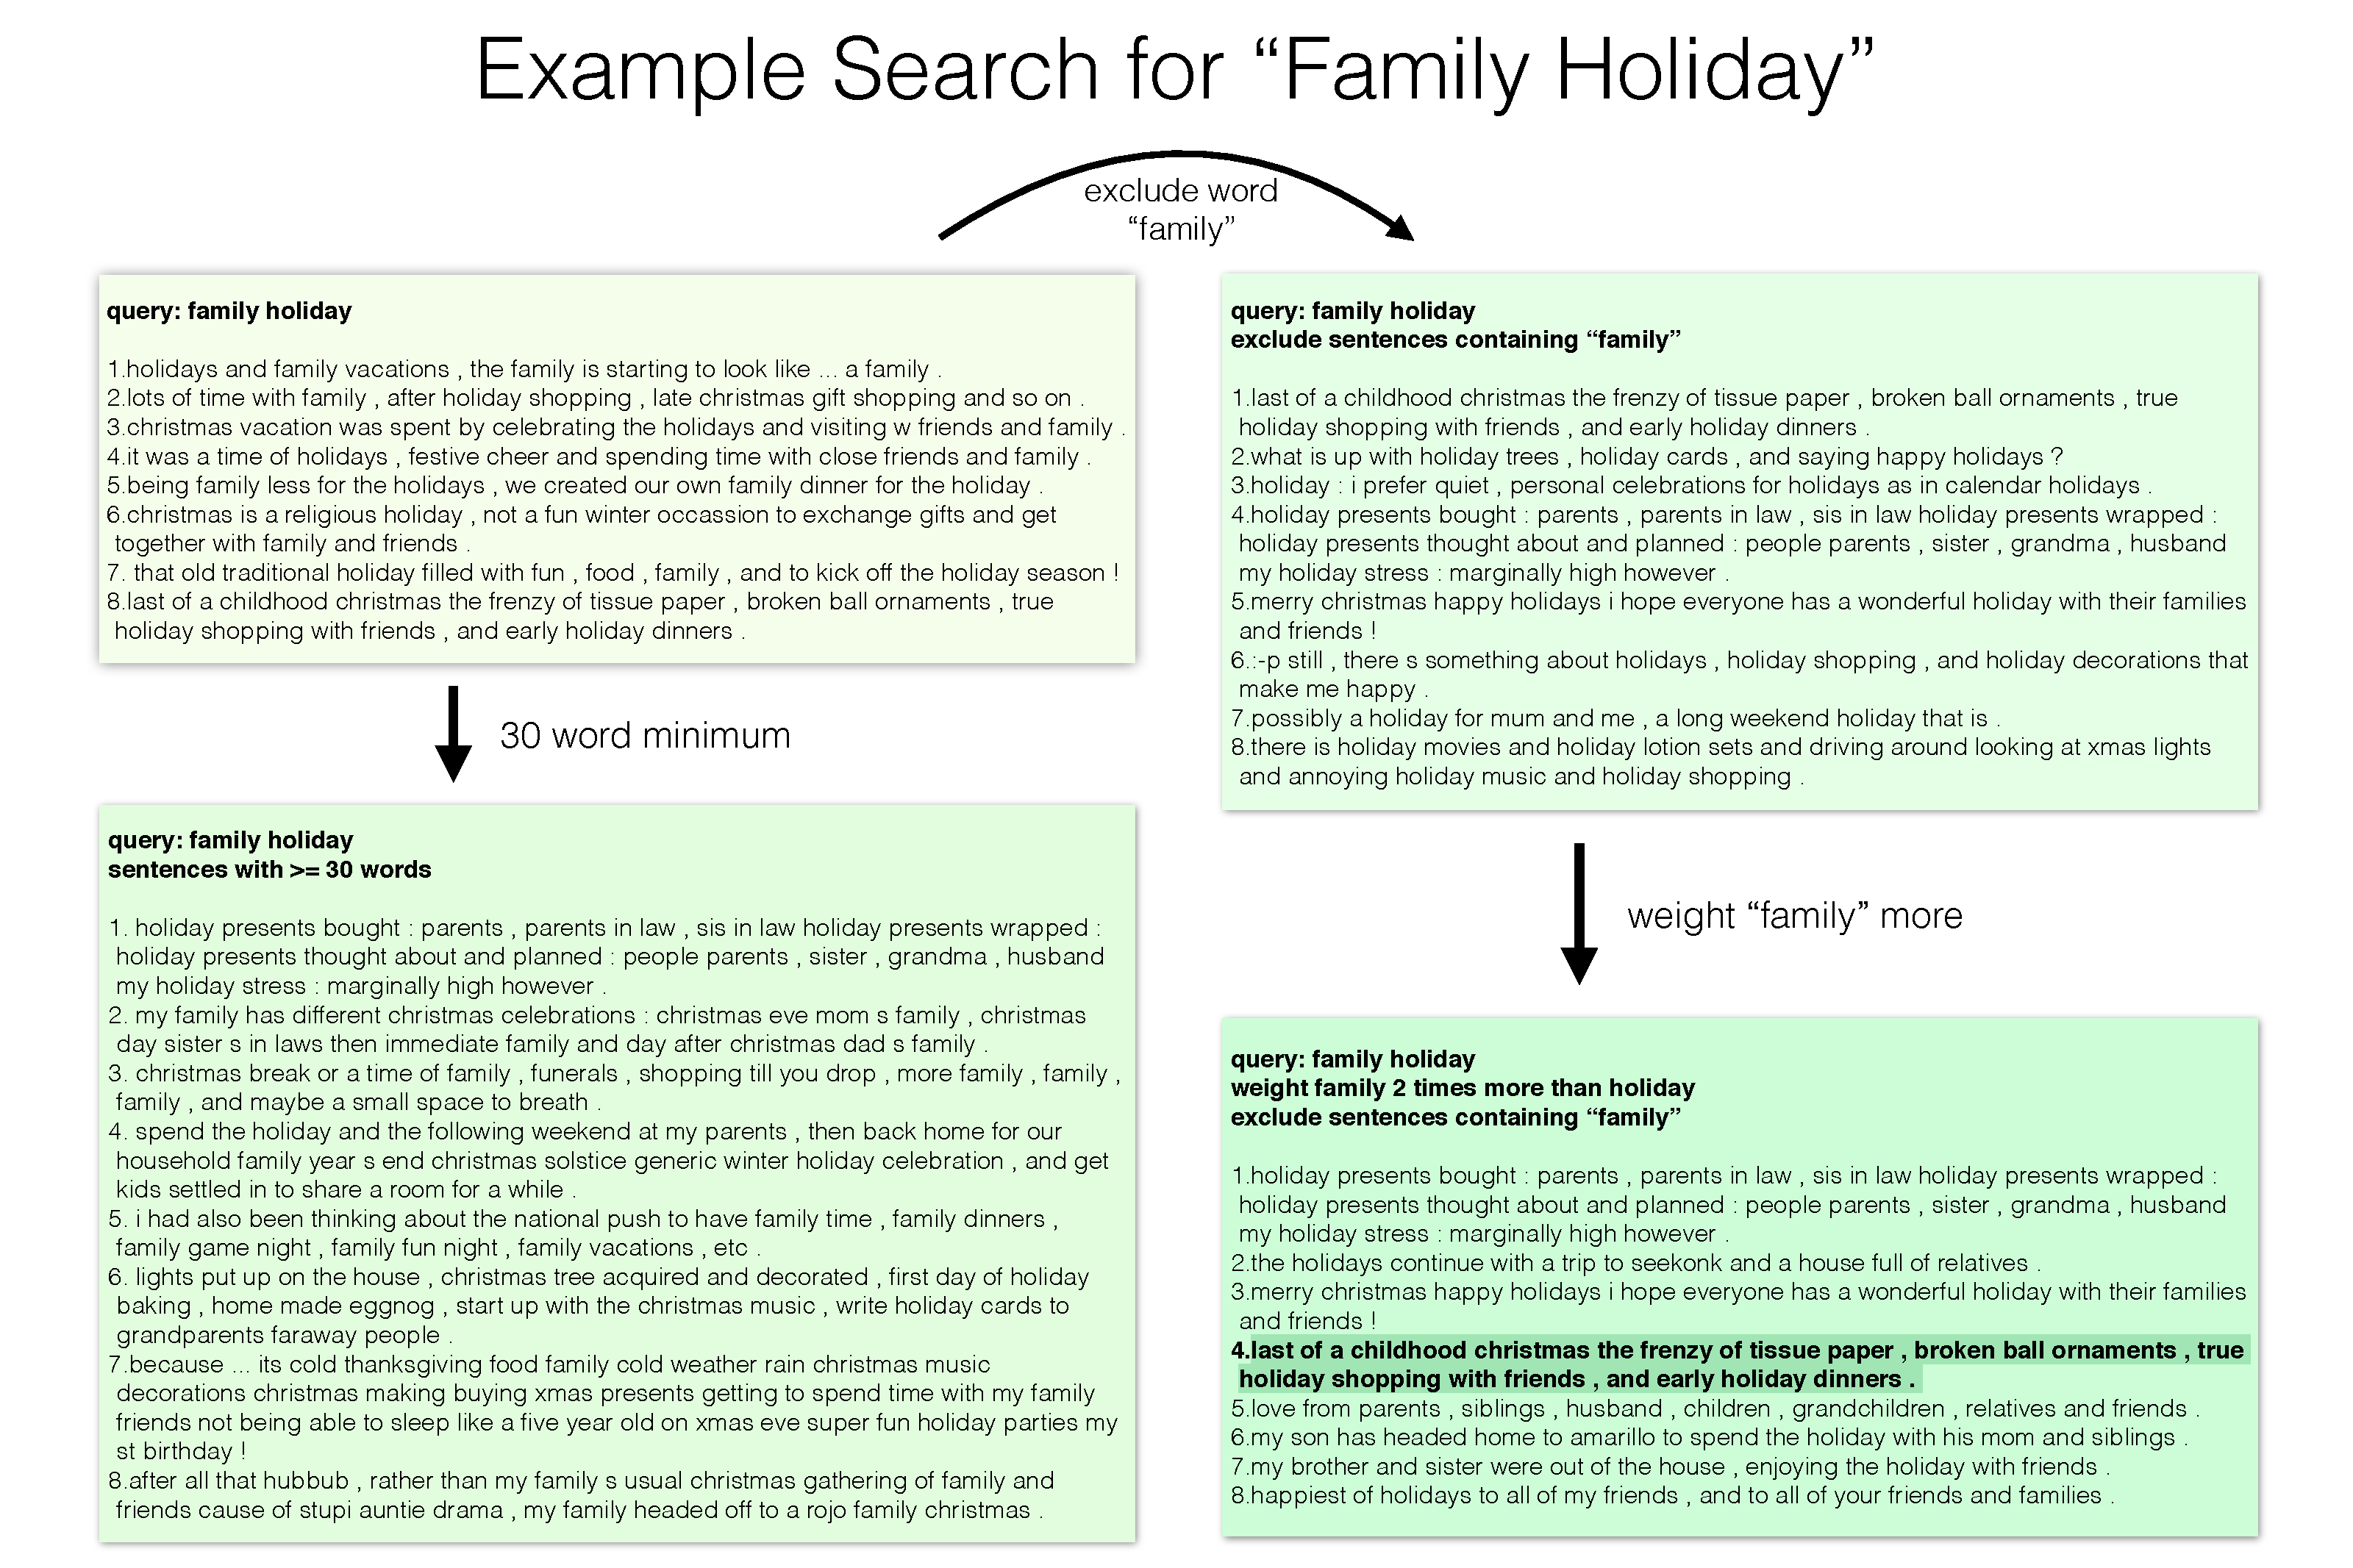
\includegraphics[width=.85\textwidth]{figures/results_1}
\caption{In this figure, we show how the filters affect the query results. 
At the top right are the top 8 results for the query ``family holiday" on the full data.  
To see more in depth responses, we can try filtering only the sentences with at least 30 words. 
This is done in the bottom left panel. 
Since we perform a semantic query, the results do not have to include our query terms. 
We can exclude the words ``family'' or ``holiday''  entirely and still get good, perhaps even better, results.
In the top right panel, we exclude the word ``family'' from the sentences in the results.
Finally, we can place more or less weight on some terms in our query. 
In the bottom right panel, we increase the weight on the word ``family'', 
to get results relating more to ``family'' than ``holiday''.  
Note that each result belongs to a full post. For instance, the highlighted result is shown in full context in Figure~\ref{fig:examplePost}. 
\label{fig:familyHolidays} }
\end{figure*}

One more interaction with a researcher focused on social relationships online. He was well versed in search models and he wanted to have an initial description of the system, which he understood well. As a matter of fact, the researcher had an inside story about a failed attempt by a commercial analysis software maker on trying to do semantic search a few years ago. He was very open to this idea and interested to see what he could find. He started with a simple query about ``family holidays'' (Figure~\ref{fig:familyHolidays} shows sample questions and responses related to this topic).

\begin{figure}[tb]
\centering 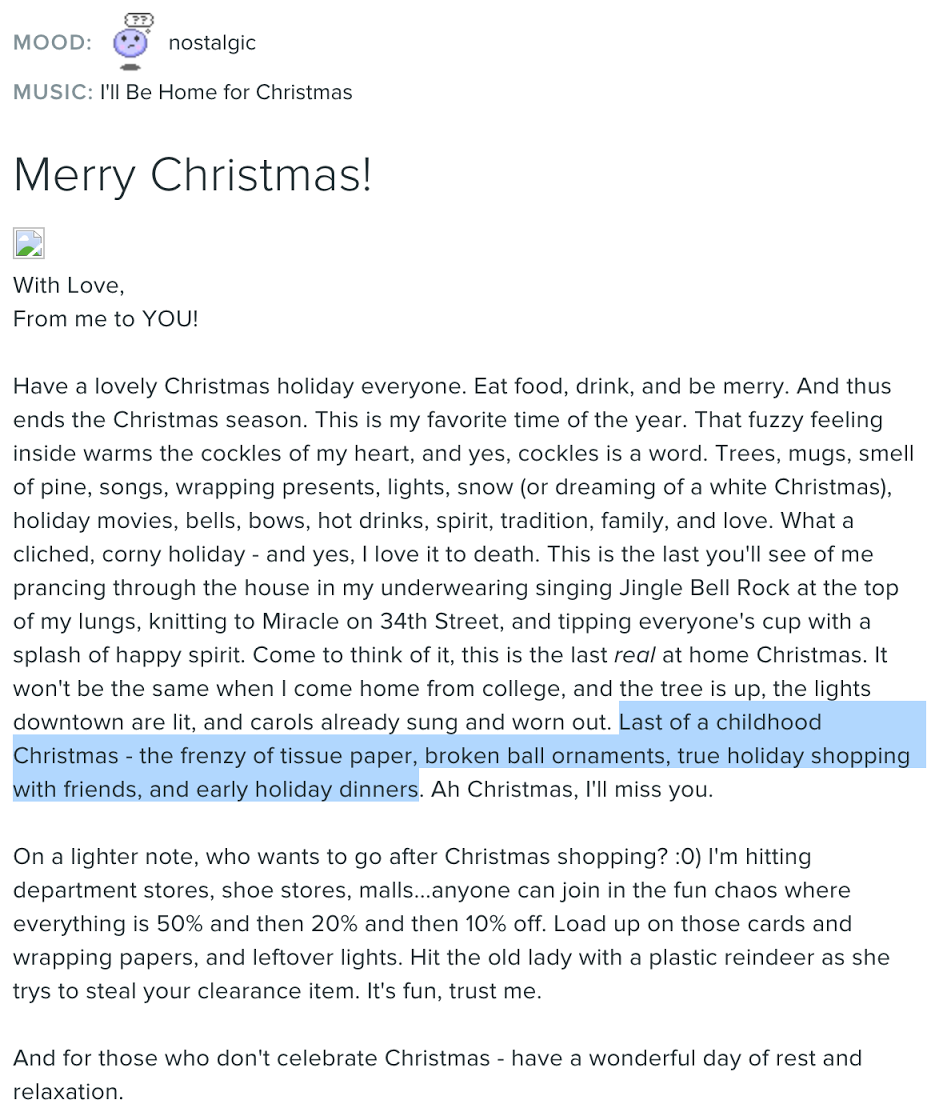
\includegraphics[width=0.4\textwidth]{figures/examplePost2} 
\caption{Actual post on LiveJournal.com corresponding to the highlighted result in Figure~\ref{fig:familyHolidays}. By viewing the full text in its original context, the interviewer is able to explore a response in even greater depth. \label{fig:examplePost}}
\end{figure}

The social relationships researcher quickly found that the data was very promising. He was very happy with the large number of responses easily available, including expressions syntactically similar to the initial query as well as others semantically close, but quite different syntactically. We visited the actual journals as well (see figure~\ref{fig:examplePost} for an example), going back and forth between the response sentences and the full journal posts. He started finding meta relations across the sentences and we came across more than one answer from the same journal. The researcher felt that the synthetic interview tool was naturally helping him to find ``genres'' of users, and thought this was a great innovation. 

\begin{quote}
{\em
This is impressive\dots the actual responses for a query are very similar\dots Ah!, if you can search for all those ``authors'', people that write about the same topic you could get something like ``genres''\dots yeah, this would be very useful
}\end{quote}

He believed that an ability to changing the unit of research from sentences to journals to genres of journals would be very valuable. The researcher also suggested that it might be interesting to store a history of queries, making a micro corpus from previous responses on which to perform additional semantic searches. He mentioned that, as the synthetic interview tool incorporates these additional complexities, some user interface (UI) tools would be necessary to make the process more tractable. 

\begin{quote}
{\em
\dots exploring text is hard... yeah, some tools like remembering my searches or some faceted search would be good, but I do not want the system to make many decisions for me, it will lead us to a ``search bubble''\dots similar to what we have not with [search engine]
}\end{quote}

He was also very impressed that among the different results he was able to find phrases that were relevant to his query, but which did not include the actual query words at all. As you can see in figure~\ref{fig:familyHolidays} the researcher searched for ``family holidays'' and found many results containing the word family, but also many that were about family without the actual word. He told us that he would like the ability to add a filter where the actual query words are excluded from the results.

\begin{quote}
{\em
\dots more than searching for the tail, it would be better to filter out ``words'' like this ``family'' word that comes many times and see only things like this one about the ``brother and the sister''?
}\end{quote}

Despite his remarks about UI tools, his biggest interest was indeed in this unique ability that our tool brought to potentially find ``genres'' of journals or groups of users, which for him was very impressive.

\subsection{Testing on more data}

By this time we had enabled a larger server with  64GB of memory to run the interactive queries on 1\% of the data. We wanted to demonstrate this new iteration to the same public health researcher, who had a mild experience the first time we had interacted. 
%We wanted to run a simple iteration only with 1\% of the data, but no filters. 
The researcher began by asking demographic questions about the data set, such as number of users, posts per user, etc. He considered this important to frame his research. He also wanted to understand better the semantic searching process and asked whether it was better to search keywords or sentences. The researcher mentioned that he is very interested in finding users that are archetypes of those who used successful strategies to lose weight and keep it low. He had also prepared a group of synonyms about eating that he wanted to search. We started searching in the lo-fi prototype just as a way to see the difference. The public health researcher began by posing the question ``i lost weight and kept it off'' with no filter and the default threshold, but found little value in the results from the lo-fi dataset. We moved then to the mid-fi prototype, which return much more relevant results for the same query. He was very impressed and wanted to see various full journal entries. He felt that some journals were excellent case studies about his topic and he even thought of other potential research that people in public policy could make. 

\begin{quote}
{\em
\dots and I think I will send this to my colleagues in the CDC, or even better get many other dissertations to other students in my department! :) \dots
}\end{quote}

The public health researcher said that he would love to see some additional features like the ability to subtract words or to get the sentences before and after the matches. Finally he said that he would like to be able to easily see the journals and select the ones he wants to work on and search on those journals alone. He also reiterated the importance of understanding the socio-demographic properties of the dataset. He was not concerned about knowing the topics embedded in the corpus, and not much interested in a predetermined diversity filter. He would not mind using it but only if he can control it.

\subsection{Mid Fidelity (Mi-Fi) Prototype}
In response to the feedback from the interviewers we implemented the additional search options (filtering, importance weighting, and minimum threshold) described Querying subsection above. We also expanded the interactive search to 1\% of the dataset. We call this the mid-fidelity (mi-fi) prototype. We now wanted to contrast our former iteration with our filters and again contacted the social networks researcher and run some of his former queries but this time with filters. 

He was delighted with the new results and made the remark that he believes that even at this level of fidelity he would be much more interested in using the tool.
\begin{quote}
{\em
\dots it is a really good tool to be able to find the chunks of data that I want to use in my studies and I would feel pretty comfortable in being able to use that [word2vec].}
\end{quote}

Finally we showed the tool to two other researchers. The first was a human computer interface researcher/designer studying online activism and multimedia communication tools for families. He found very little merit in the data for the activism topic, likely because his particular research topics were more modern than our dataset. We will later see that when we run the queries on 100\% of the data, the value of the results improces. Even with the mi-fi model, he did find some references that he found interesting once he adapted his search strategy from keywords to more colloquial expressions (such as ``please sign my petition''). At this point he made a very important remark. He found that he had to completely change his search paradigm when using the synthetic interview tool, moving away from the example based queries that are successful with traditional keyword search engine queries and towards semantically meaningful questions. 

\begin{quote}
{\em
I think the problem might be when you think about a search or a query tool we are way to much biased by our daily search experience, ``all about keywords'' but it seems to me that this, for this to work, you have to give an example.
}\end{quote}

\begin{figure*}[ht!]
\centering 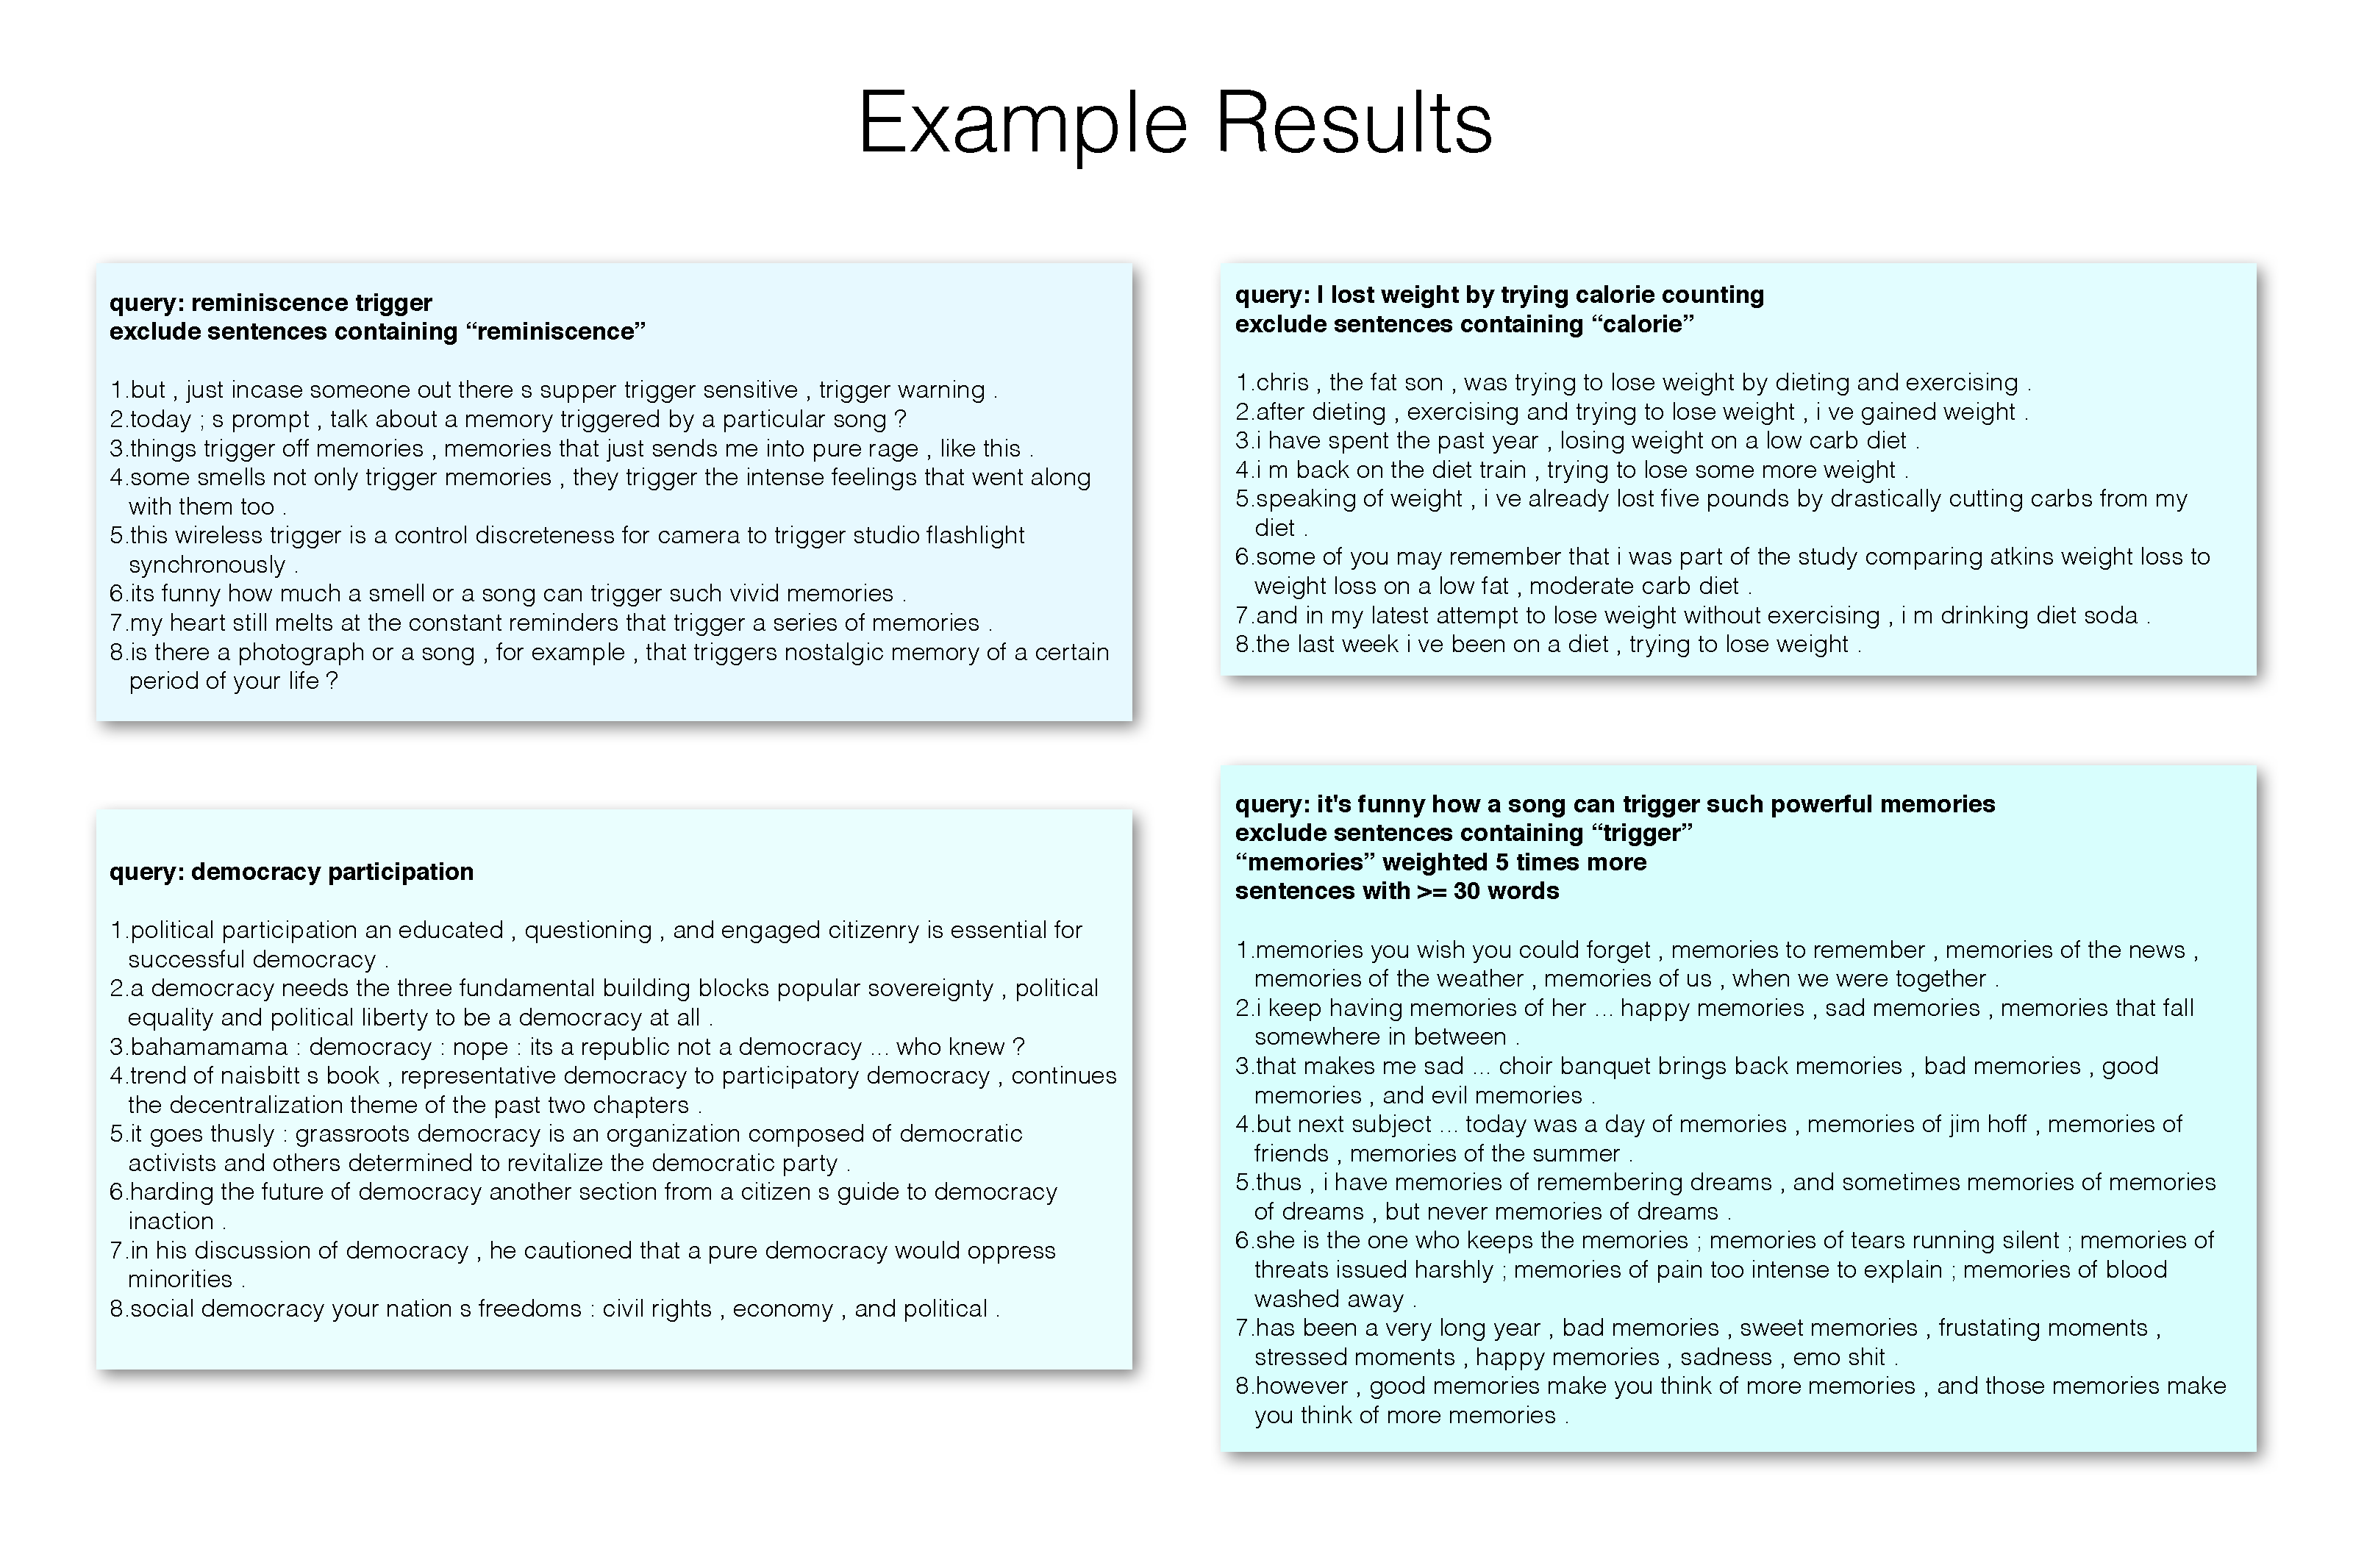
\includegraphics[width=\textwidth]{figures/results_2} 
\caption{Some example queries and results using our method.  \label{fig:reminiscenceTriggers}}
\end{figure*}

When he started searching for the information about a previous research topic, ``reminiscence trigger,'' the human computer interaction researcher was very happy with the results results (see figure~\ref{fig:reminiscenceTriggers} for some examples). He said that the top results validated his past findings, from traditional research processes, that songs and smells are extremely triggers of reminiscence. He believed that synthetic interviewing has potential to support research at a formative phase as well as during refinement of the hypothesis. With more information about the population, the synthetic interview process could even become a useful formal tool.

Finally, we closed our interviews with a law sociologist researching access to justice. The initial search results were quite peculiar because of the formal phrasing of her queries. When searching for ``presence in court'' many answers were about tennis courts. However when we added the filter to eliminate the word ``ball'' from the results the answers were much better and she found many interesting quotes about the judiciary system. She reiterated the point of previous researchers that access to detailed demographic information is a key element to make the tool viable. Without that it would be very hard to use it in publications.

% Edited to here. -Cory

\begin{quote}
{\em
I believe that I can use this tool in two moments. In the beginning of my research when I want to decide which issue I will talk about say I will try to figure out what is going on, what people are talking about, what are the main issues that are going on. I can bring one issue that is interesting to help me make the right question. It's nice to see what people are talking [about]. I can then build the question to be tested. And then I see another time to use it when I want to make real research with people and I don't have enough money or have enough time to go to the field, it will make it easier and more applicable to make research with people. 
}\end{quote}

However, the law sociologist believed that even without those key validation elements, the tool would be very helpful during the initial phase of the hypothesis formulation. She believed that the tool itself would be a great way to save money and time instead of going ``door to door'' at the early stages. She mentioned that for some of her projects, e.g. in the favelas of Rio de Janeiro, she was not even able to go to the field as it was too dangerous and she was forced to rely on secondary sources, like police or judiciary documents, to study the process of pacification within the favelas. She believed that if the synthetic interview tool could be applied to a corpus of data containing posts from such areas, this tool would allow her direct contact with the people's voice. Even in more accessible areas, she believe the simple ability to search quickly through what the people think about a topic is very compelling. 

\begin{quote}
{\em
I had experience in Brazil because my field was impossible, so I decided to make research where I could have access available. So I decided to make a new social system. It was impossible to have people to classify the favelas, so I went to the judicial system database for the jurisprudence so I could make a research through the point of view of the institution.
}\end{quote}

The law sociologist also expressed that she was eager to use the tool as soon as possible for her current research topic.

%\subsection{Full capacity Simulation}
%We implemented an off-line search option at full capacity (100\%). Results from this implementation are explained in the next section.

\section{Results}

\begin{figure*}[htb]
\centering 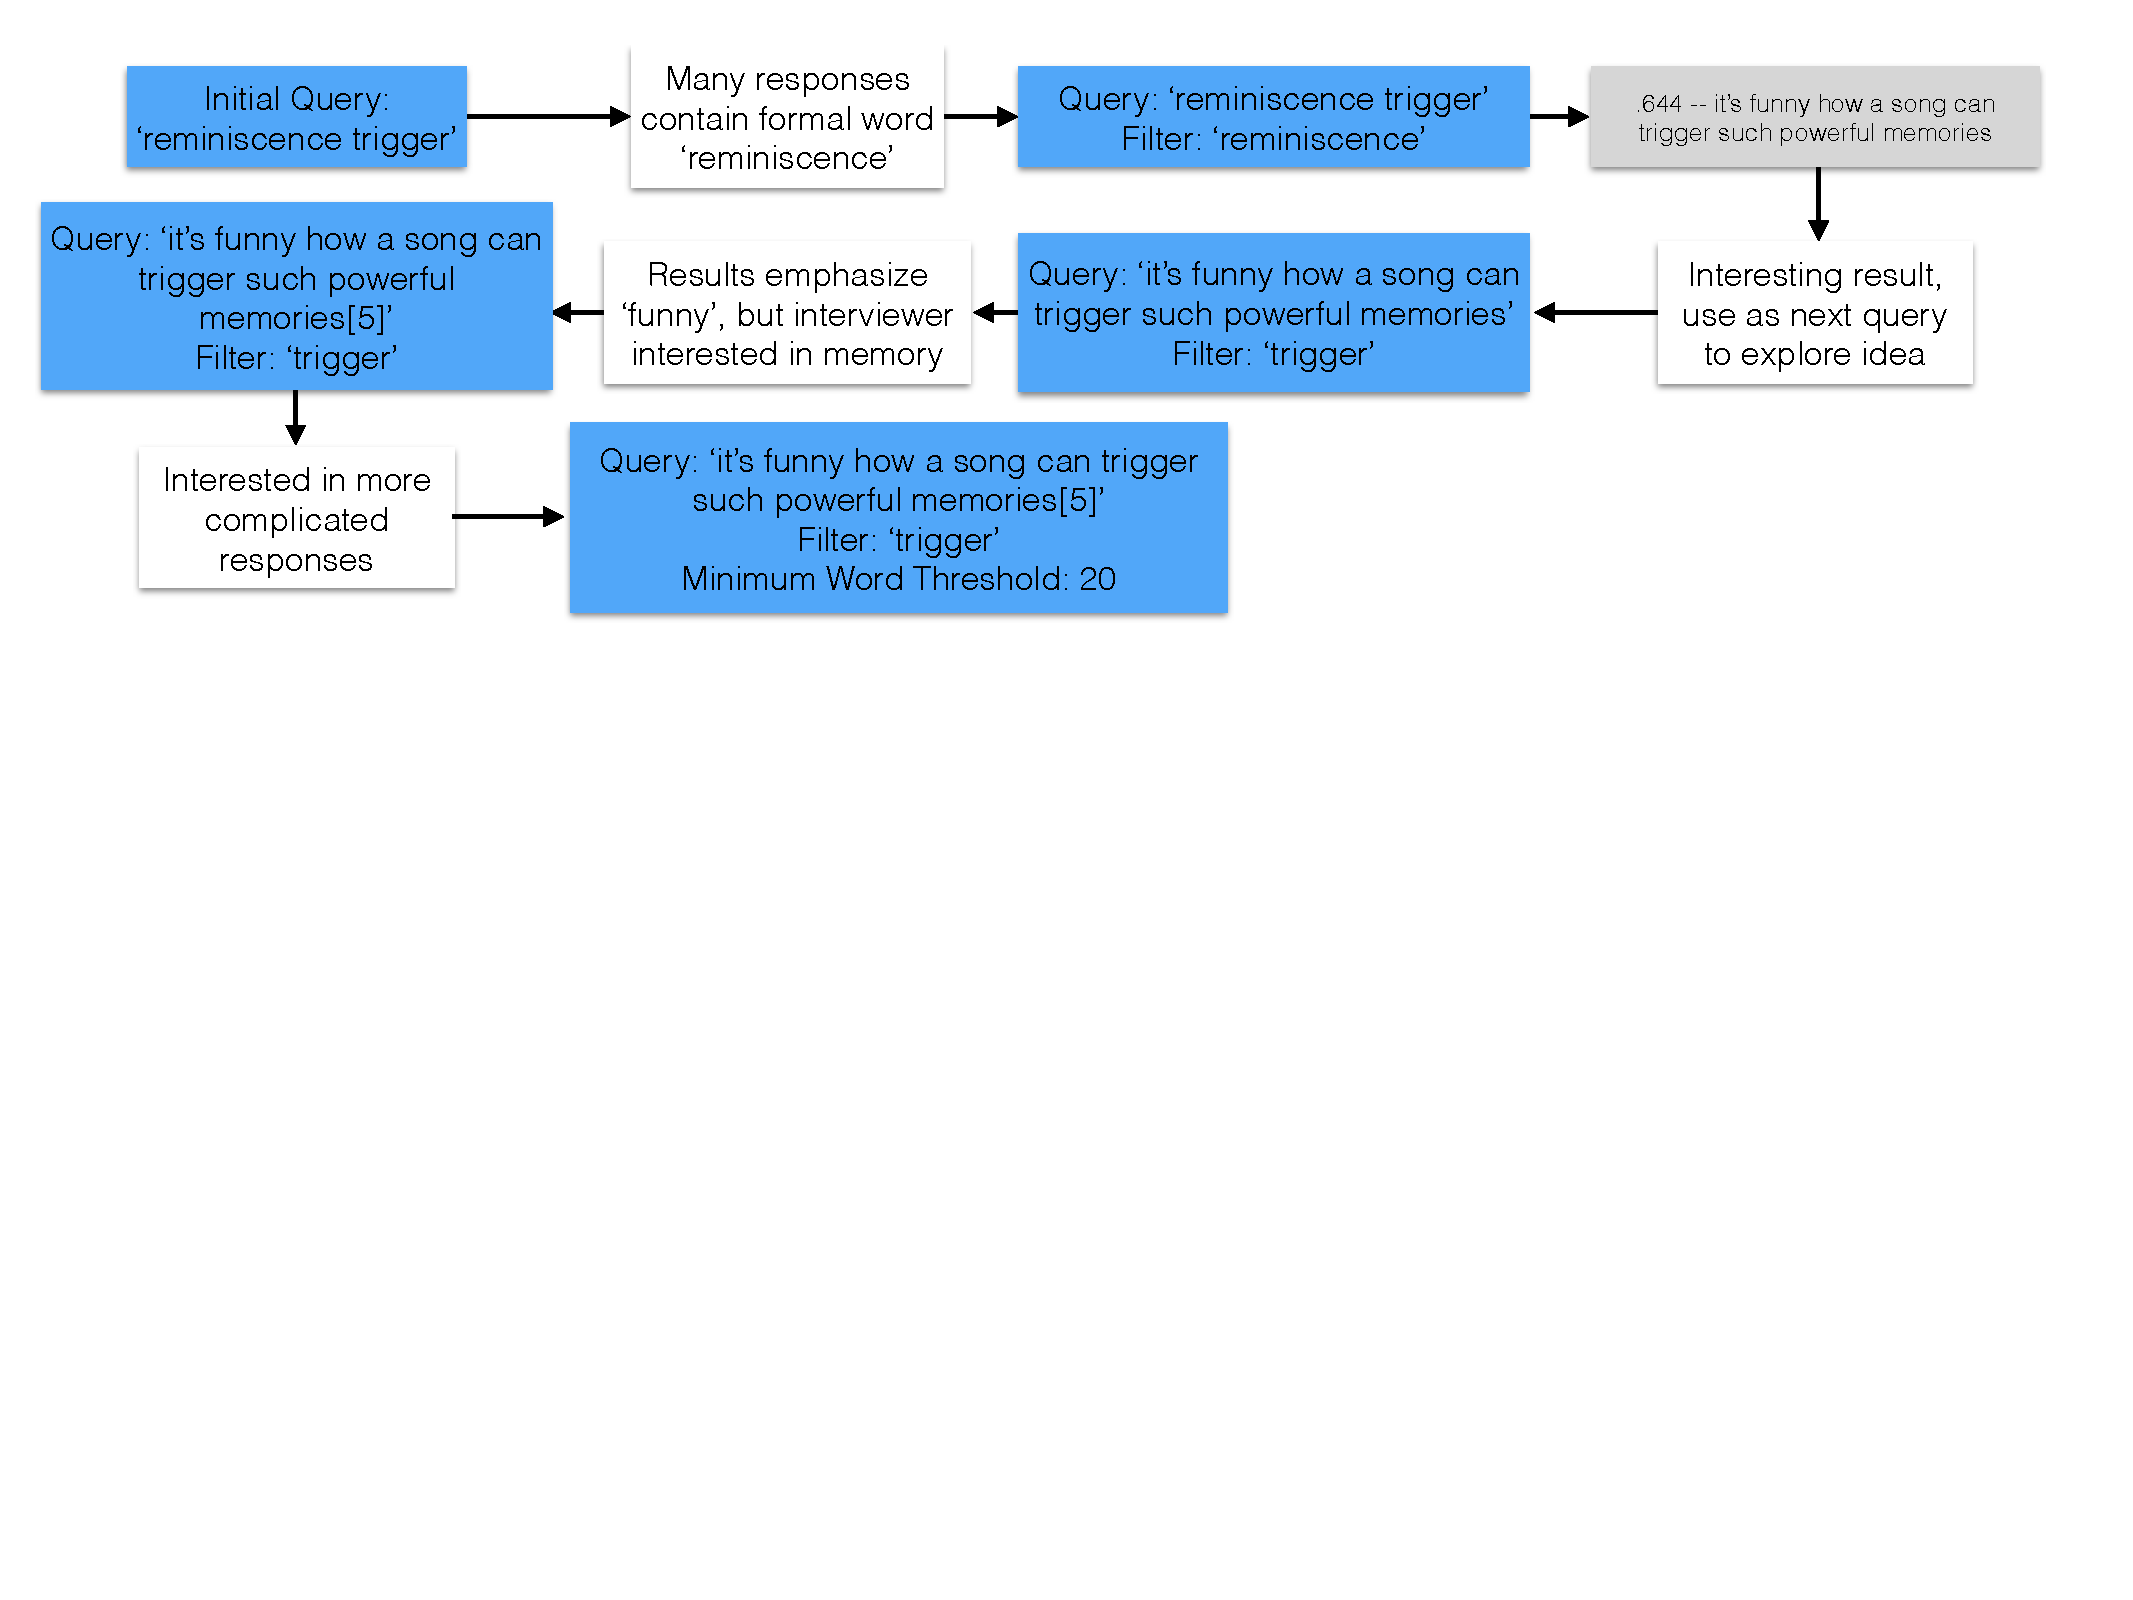
\includegraphics[width=0.8\textwidth]{figures/InterviewFlow.pdf} 
\caption{Example of how the synthetic interview questions evolve in response to the returned answers based on a real synthetic interview. This example is linear for simplicity of presentation, but the interviewer can easily follow a line of questioning and then return to an earlier query as many times as desired. The flow is somewhat analogous to semi-structured interviewing, where interviewers must modify their line of questioning on the fly to respond to answers received.}
\end{figure*}

%\begin{figure}[tb]
%\centering 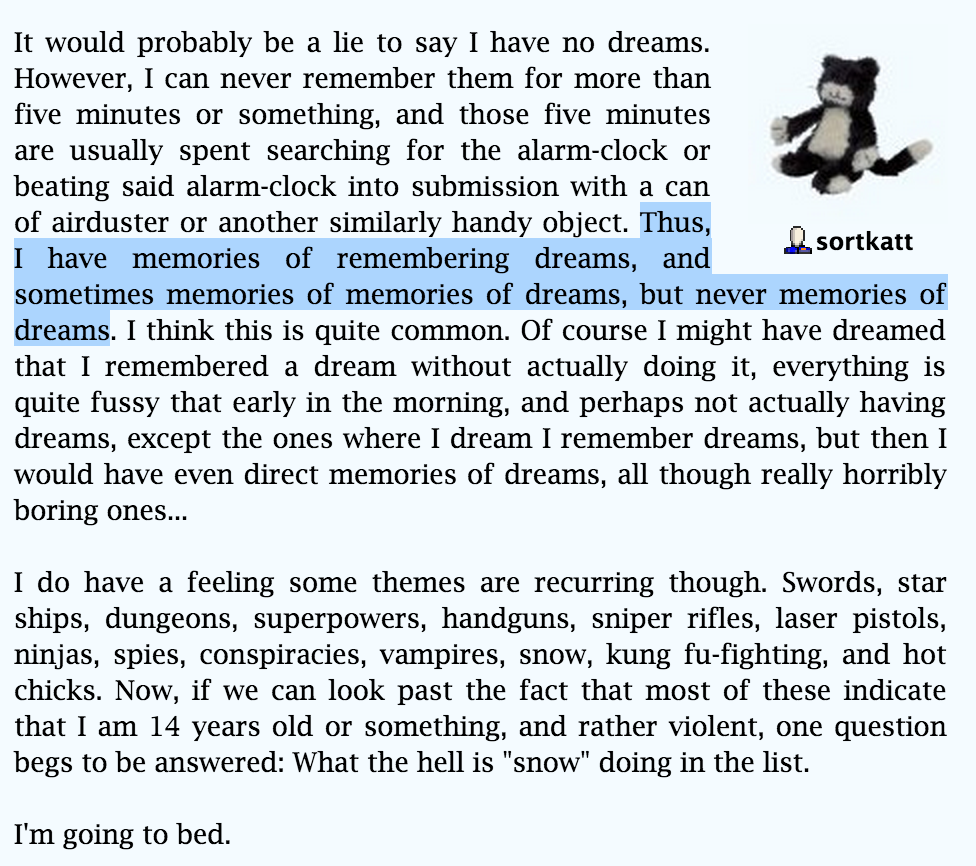
\includegraphics[width=0.45\textwidth]{figures/examplePost1} 
%\caption{Actual post on LiveJournal.com corresponding to the highlighted result in Figure ?. }
%\end{figure}


\subsection{Bridging Formal with Informal Language}
By applying the discussed SGNS Google News-trained word2vec model, on our LiveJournal sparse matrix, we simulate a bridge between formal semantics and vast compilation of informal anecdotes. To explore the potential advantage of such combination, we extended this tool to several academic researchers. As stated by an online activism researcher, this tool is unlike others in that it is ``not all about keywords''. Instead, the researcher states that he ``can also profit from [our tool]'' by simply ``thinking of examples to search on''. Unlike traditional searching, querying on an example can return ``instances of people saying similar things''. 

The obtained responses demonstrate one of many applications of generating synthetic interviews. Such application inspires curiosity of finding ways to expand its relevance beyond an academic setting. 

\subsection{Model versus Corpus}
While a majority of our trials yielded positive results, we cannot ignore the remaining minority that did not echo similar success. One researcher voiced that because ``the corpus is LiveJournal, [most authors] post about topics such as food, love, and marriage'', however there ``would not be [entries] on topics like physics''. 

Such subpar retrievals bring attention to the parameters that may impact the quality of our queries. There are two major variables we chose in our implementation: the text corpus for training (Google News) and the actual corpus of text we are querying on (LiveJournal). In many cases, we found our choices to be sufficient; in an academic context, we can imagine researchers to seek answers to formal questions, in order to trigger responses that may be colloquial anecdotes. However, as demonstrated by the above response, an appropriate training-query corpus pair for one category may not necessarily be optimal for another category.

To find such pair that is appropriate for a desired topic, we recognize that there are distinct trends and biases from corpus to corpus. In our case, we observed that a dominating majority of the posts were in the form of journal entries, as LiveJournal was designed for that purpose. Additionally, most authors were within the 17-25 age group.


\section{Conclusions}


\section{Acknowledgments}


\bibliographystyle{SIGCHI-Reference-Format}
\bibliography{destressCHI}

\end{document}